
\chapter{Stato dell'arte}
Al fine di poter operare correttamente, il Power Stack deve gestire e monitorare la potenza assorbita, le frequenze e le temperature di processori all'interno dei sistemi ad alte prestazioni. Questo deve poter essere fatto anche a diversi livelli come intero sistema, singoli nodi e singoli elementi all'interno dei nodi. E' quindi necessario poter 
\setlength{\intextsep}{1pt} 
\begin{wrapfigure}{r}{0.5\textwidth}
    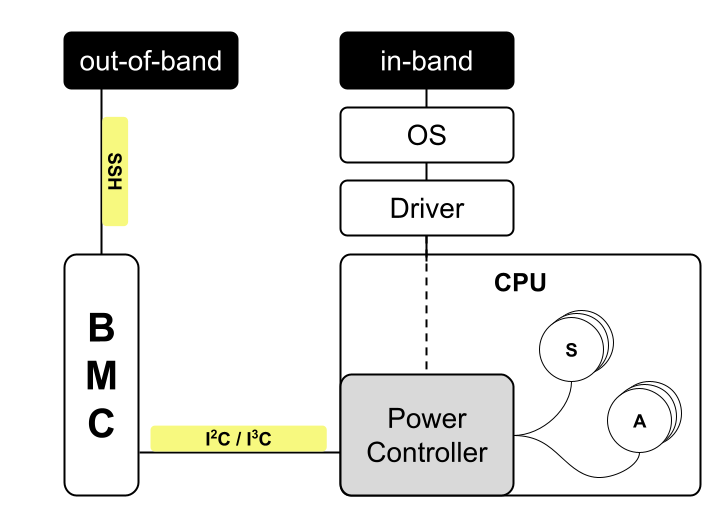
\includegraphics[width=0.5\textwidth]{img/SoA.png}
    \centering
    \caption{Differenza tra le interfacce in-band e out-of-band}\label{fig:SoAinoutband}
\end{wrapfigure}
accedere agli attuatori e sensori presenti nei core sia in modo diretto che da ''remoto''. Normalmente per farlo ci sono due vie disponibili basate su interfacce differenti:
\begin{itemize}
    \item in-band
    \item out-of-band
\end{itemize}
% Nella figura~\ref{fig:SoAinoutband} viene schematizzata la differenza tra le due interfacce disponibili. 
Nella figura~\ref{fig:SoAinoutband} viene schematizzato l'accesso ai dispositivi hardware che si occupano della gestione del power management su sistemi HPC. Sarebbe in realtà possibile accedere a questi componenti anche tramite altri meccanismi specifici, ad esempio la mappatura in memoria condivisa dei componenti hardware, tuttavia a causa della loro natura altamente specializzata, tali approcci non saranno considerati nell'ambito di questa tesi.

% I servizi in-band vengono forniti alle applicazioni e ai sistemi operativi in esecuzione negli elementi di elaborazione del chip e sono composti da: (i) governor dedicati alla potenza e telemetria correlata alla potenza a livello di sistema operativo; (ii) un'interfaccia dedicata per consentire alle applicazioni e ai tempi di esecuzione del modello di programmazione di specificare suggerimenti e prescrizioni per la gestione della potenza; (iii) un'interfaccia dedicata al Sistema e alla Gestione delle Risorse per supportare il capping della potenza a livello di CPU e nodo, nonché per gestire il compromesso tra Throughput ed Efficienza Energetica. I servizi out-of-band vengono forniti all'amministratore di sistema e agli strumenti di gestione del sistema tramite il Controller di Gestione della Scheda (BMC). Questi servizi consistono nella telemetria di potenza out-of-band, nel capping di potenza a livello di sistema e nella affidabilità e assistenza.

% (ii) off-chip ai Moduli Regolatori di Tensione (VRM) che alimentano il chip, gli altri componenti a bordo e il Controller di Gestione della Scheda (BMC).

\section{Servizi in-band}
I servizi in-band accedono alle risorse hardware tramite codice che esegue sul processore stesso. Questi sono resi possibili da infrastrutture come CPUfreq\cite{CPUfreq} o RAPL\cite{RAPL} (per architetture intel) che tramite dei driver, espongono a livello utente le manopole per gestire e monitorare frequenze e informazioni della cpu. Questo passaggio viene reso possibile da interfacce fornite dal sistema operativo. Queste ultime possono essere gestite in automatico in base al carico di sistema, in risposta ad eventi ACPI oppure in modo manuale. Una volta scelti i driver come \emph{ACPI CPUfreq driver} o \emph{Intel P-state} (in sistemi intel) è possibile scegliere tra diversi governors (o governatori) disponibili, che permettono di agire con delle policy differenti.
Per esempio \emph{CPUfreq} fornisce diversi governors per soddisfare diversi tipi di situazioni, come:
\begin{itemize}
    \item performance: forza la CPU ad eseguire alla frequenza massima disponibile;
    \item powersave: forza quella minima;
    \item ondemand: comportamento dinamico in base all'utilizzo di sistema;
    \item userspace: permette ai selezionati user-space di impostare la frequenza; 
    \item conservative: come ondemand ma con più inerzia al cambiamento;
\end{itemize}

\begin{figure}[H]
    \centering
    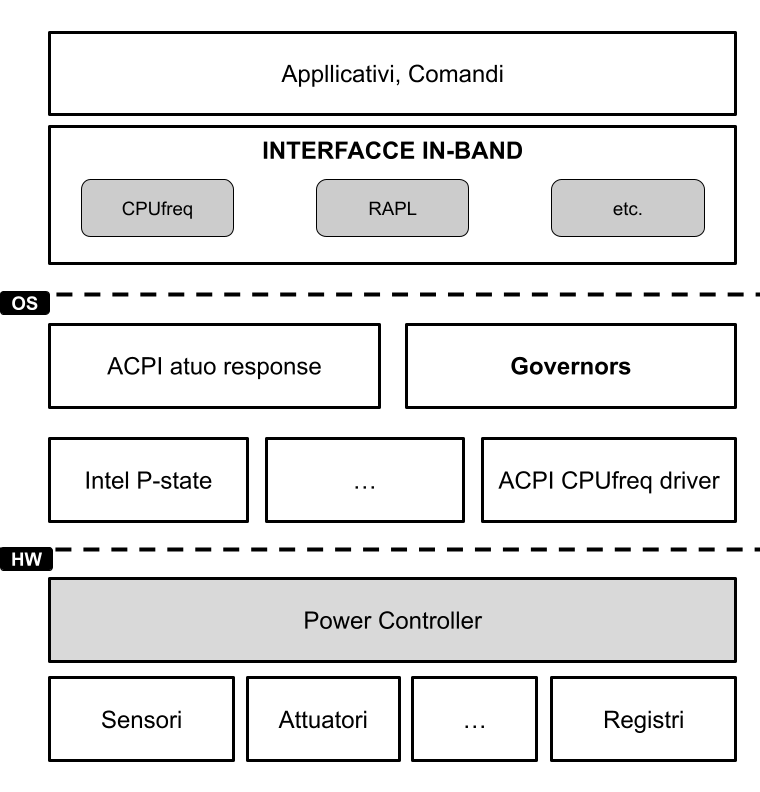
\includegraphics[width=0.65\textwidth]{img/in-band.png}
    \caption{Struttura interfacce in-band: divise su più livelli tra cui Sistema Operativo (SO) e Hardware (HW)}\label{fig:inband}
\end{figure}

Il vantaggio di usare queste interfacce è che permettono di operare in real-time ed in modo dinamico. I lati negativi invece risiedono nelle stesse peculiarità di questi strumenti, ovvero che possono ottenere le informazioni solamente nei core sui quali i processi vengono eseguiti. 

% E' reso possibili tramite degli specifici driver (intel\_pstate) che comunicano con i componenti hardware sul chip. Diversamente \textbf{Intel Power Governors} utilizza le interfacce proprietarie (RAPL) con cui monitora potenza ed energia a livello di sistema.
% Entrambi questi strumenti hanno necessità di componenti Hardware dedicati come i power knob (manopole per la gestione della potenza) e sensori che permettono di monitorare temperature e tensioni.
% I servizi in-band sono molto flessibili e permetto di operare in real-time ed in modo dinamico. Infatti interagendo con l' Hardware e passando tramite il sistema operativo, sono necessari semplici chiamate e comandi per controllare questi strumenti.

\section{Servizi out-of-band}
Contrariamente alle interfacce in-band, i servizi out-of-band fanno utilizzo di \emph{sidechannels} ovvero canali di accesso alternativi per ottenere i dati richiesti. Questo meccanismo permette a processi esterni\footnote{In esecuzione su processori diversi dai quali si vuol reperire dati} di accedere alle informazioni contenute nel processore che si vuole analizzare. Per di più questo permette di monitorare i componenti anche quando ci sono errori ed eccezioni che normalmente bloccherebbe il servizio. Un componente tra i più importanti che svolge questa funzione è il Baseboard Management Controller (BMC), solitamente un micro-controllore animato da sistemi embedded linux, e accessibile tramite un canale separato (solitamente provvisto di una propria interfaccia di rete e/o bus specifici). Il suo principale scopo è quello di monitorare in modo dettagliato lo stato di tensioni, temperature, ventole e prestazioni dei processori e fornire contemporaneamente servizi di power capping sia a livello di sistema (non possibile tramite le interfacce in-band) che di singoli processori.
Recentemente alcuni produttori di BMC introducono anche dispositivi FPGA da affiancare al BMC per aumentarne le capacità.
% \vfil
\begin{figure}[H]
    \centering
    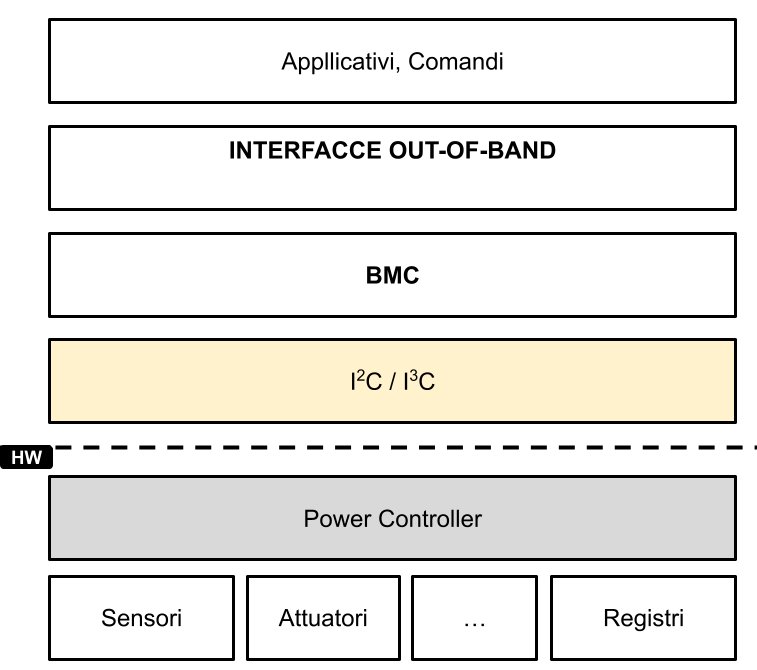
\includegraphics[width=0.75\textwidth]{img/out-of-band.png}
    \caption{Struttura interfacce out-of-band} 
    \label{fig:out-of-band}
\end{figure}


\section{Interfacce di alto livello}
Nel corso degli anni con l'obbiettivo di ottimizzare e automatizzare l'interazione con questi meccanismi hardware sono stati sviluppati diversi software di più alto livello che utilizzano sia interfacce in band che interfacce out of band. Si possono ricordare i più famosi: \emph{Variorum} (LLNL), \emph{GEOPM} (Intel)\cite{GEOPM}, e \emph{HDEEM} (Atos)\cite{HDEEM}. Tutti questi rappresentano però un tentativo di fornire una soluzione ad un sottoinsieme di problemi per la gestione dell'energia o potenza, piuttosto che ad un software con visione globale di Power Management per sistemi di calcolo ad alte prestazioni. %MANCANZA DI VISIONE GLOBALE!!!


\section{Modello di power stack} %Componenti power stack
Con Power Stack si intende un insieme di software che cooperando riescono a fornire ad applicazioni, utenti e amministratori la gestione completa del Power Management. Una volta definito il problema, ed i componenti che possono essere utilizzati, è possibile definire un modello di interazione e responsabilità dei vari attori. Di seguito vengono riportati quelli che sono i ruoli necessari al fine di coordinare un sistema HPC dall'allocazione di un applicativo, fino alla gestione delle tensioni. 
\begin{itemize}
    \item Workflow engine (WE)
    \item System Power Manager (SPM)
    \item Job Manager (JM)
    \item Job Scheduler (JS)
    \item Resource Manager (RM)
    \item Node Manager (NM)
    \item Monitor (M)
\end{itemize}
%TODOV aggiungi i tipi di informazioni che si scambiano, per facilitare nel modello la realizzazione

\subsection{Workflow engine}
Il workflow o \emph{flusso di lavoro} è un insieme task che devono essere svolti per risolvere un determinato problema. Il workflow engine si occupa di analizzare le dipendenze e le richieste di risorse di ogni workflow e decide dinamicamente come dividerlo nei jobs che verranno successivamente assegnati al Job Scheduler. %Si occupa quindi di analizzare ed assegnare i diversi task a chi poi va ad eseguirli.

\subsection{System Power Manager}
Il System Power Manager si occupa di comunicare con tutti i Node Manager all'interno del sistema, per impostare eventuali limiti di potenza. Questi ultimi vengono solitamente impostati manualmente dagli amministratori di sistema, oppure in modo automatico comunicando con altri attori, come monitor e Node Manager. Una volta fissati i limiti, vengono monitorati i dati relativi a potenza ed energia, e controlla di conseguenza i budget, e la \emph{user-fairness}.
\subsection{Job scheduler}
%Il System Manager
Il job scheduler dopo aver ricevuto come input un insieme di jobs li schedula all'interno del sistema, e in modo indicativo decide quando schedulare ogni job, su quale nodo, e con quale power budget. In particolare la serie di compiti che si trova a svolgere è il seguente:
\begin{enumerate}
    \item L'utente schedula i jobs da svolgere in una o più code, definite dal Workflow Engine.
    \item Il Job scheduler esamina tutte le code e i job in esse contenute, e decide dinamicamente, quale sarà l'ordine di esecuzione, e il tempo massimo in cui viene assegnata una risorsa.
\end{enumerate}
Generalmente si cerca di ottimizzare alcune caratteristiche come il tempo di utilizzo del sistema oppure l'accesso veloce alle risorse per alcuni sottoinsiemi di jobs. Inoltre le code definite, possono avere diverse priorità o può essere ristretto l'accesso a soli alcuni utenti.% I job scheduler possono condividere un nodo anche con più utenti contemporaneamente, in base all'utilizzo che devono farne. Per farlo il nodo viene allocato e diviso in partizioni virtuali, che vengo ''sciolte'' una volta finiti i job in esecuzione. Questo permette di utilizzare al massimo i componenti messi a disposizione dal sistema HPC.

\subsection{Resource Manager}
Per riuscire a svolgere questo lavoro il Job Scheduler interagisce con uno o più Resource Manager\footnote{A volte per questo il Job Manager ed il Resource Manager vengono collassati in un unico componente}. Questi sono software che hanno il compito di dividere (o condividere) e orchestrare le risorse computazionali e fisiche del sistema HPC. Queste risorse includono diversi componenti:
\begin{itemize}
    \item Nodi
    \item Processori
    \item Memorie
    \item Dischi
    \item Canali di comunicazione (compresi quelli di I/O)
    \item Interfacce di rete 
\end{itemize}
Per esempio quando un Job Scheduler deve eseguire un job, richiede al RM di allocare core, memorie, dischi e risorse di rete in base alle specifiche di esecuzione del job.
Infine in alcuni casi il RM è anche responsabile di gestire la distribuzione elettrica e raffreddamento di alcune parti dei centri di calcolo\cite{ResourceManager}.

\subsection{Job Manager}
Lo scopo del job manager è quello di effettuare ottimizzazioni job-centriche considerando le prestazioni di ogni applicazioni, il suo utilizzo di risorse, la sua fase e qualsiasi interazione dettata da ogni workflow in cui è presente. In breve il job manager decide i target delle manopole del Power Management, come (i) CPU power cap, (ii) CPU clock frequency oltre ad eseguire ottimizzazione del codice.

\subsection{Node Manager}
Il node manager fornisce accesso ai controlli e monitoraggio hardware a livello del nodo. Volendo permette anche di definire delle policy di power management. Ha infine lo scopo di preservare integrità, sicurezza del nodo sia in termini informatici che fisici.

\subsection{Monitor}

Il monitor è responsabile di collezionare tutte le metriche in-band e out-of-band che riguardando prestazioni, utilizzo e stato delle risorse, potenza ed energia.
Tutto questo deve essere fatto con il minor impatto possibile sul sistema dove sta agendo, collezionando, aggregando e analizzando le metriche e dove necessario, scambiandole ad altri attori. A sua volta il \emph{Monitor} è scomponibile in tre sotto-moduli:
\begin{itemize}
    \item Gestione Firma che genera una firma che identifica univocamente il job; 
    \item Estimatore che valuta le proprietà dei job o dello stato del sistema usando la firma generata precedentemente;
    \item Dashboard che fornisce le funzionalità da mostrare agli sviluppatori.
\end{itemize}


Per concludere viene mostrato uno schema in figura~\ref{fig:powerstackscheme} che mostra gli attori e le possibili interazioni che possono avere.
\begin{figure}[H]
    \centering
    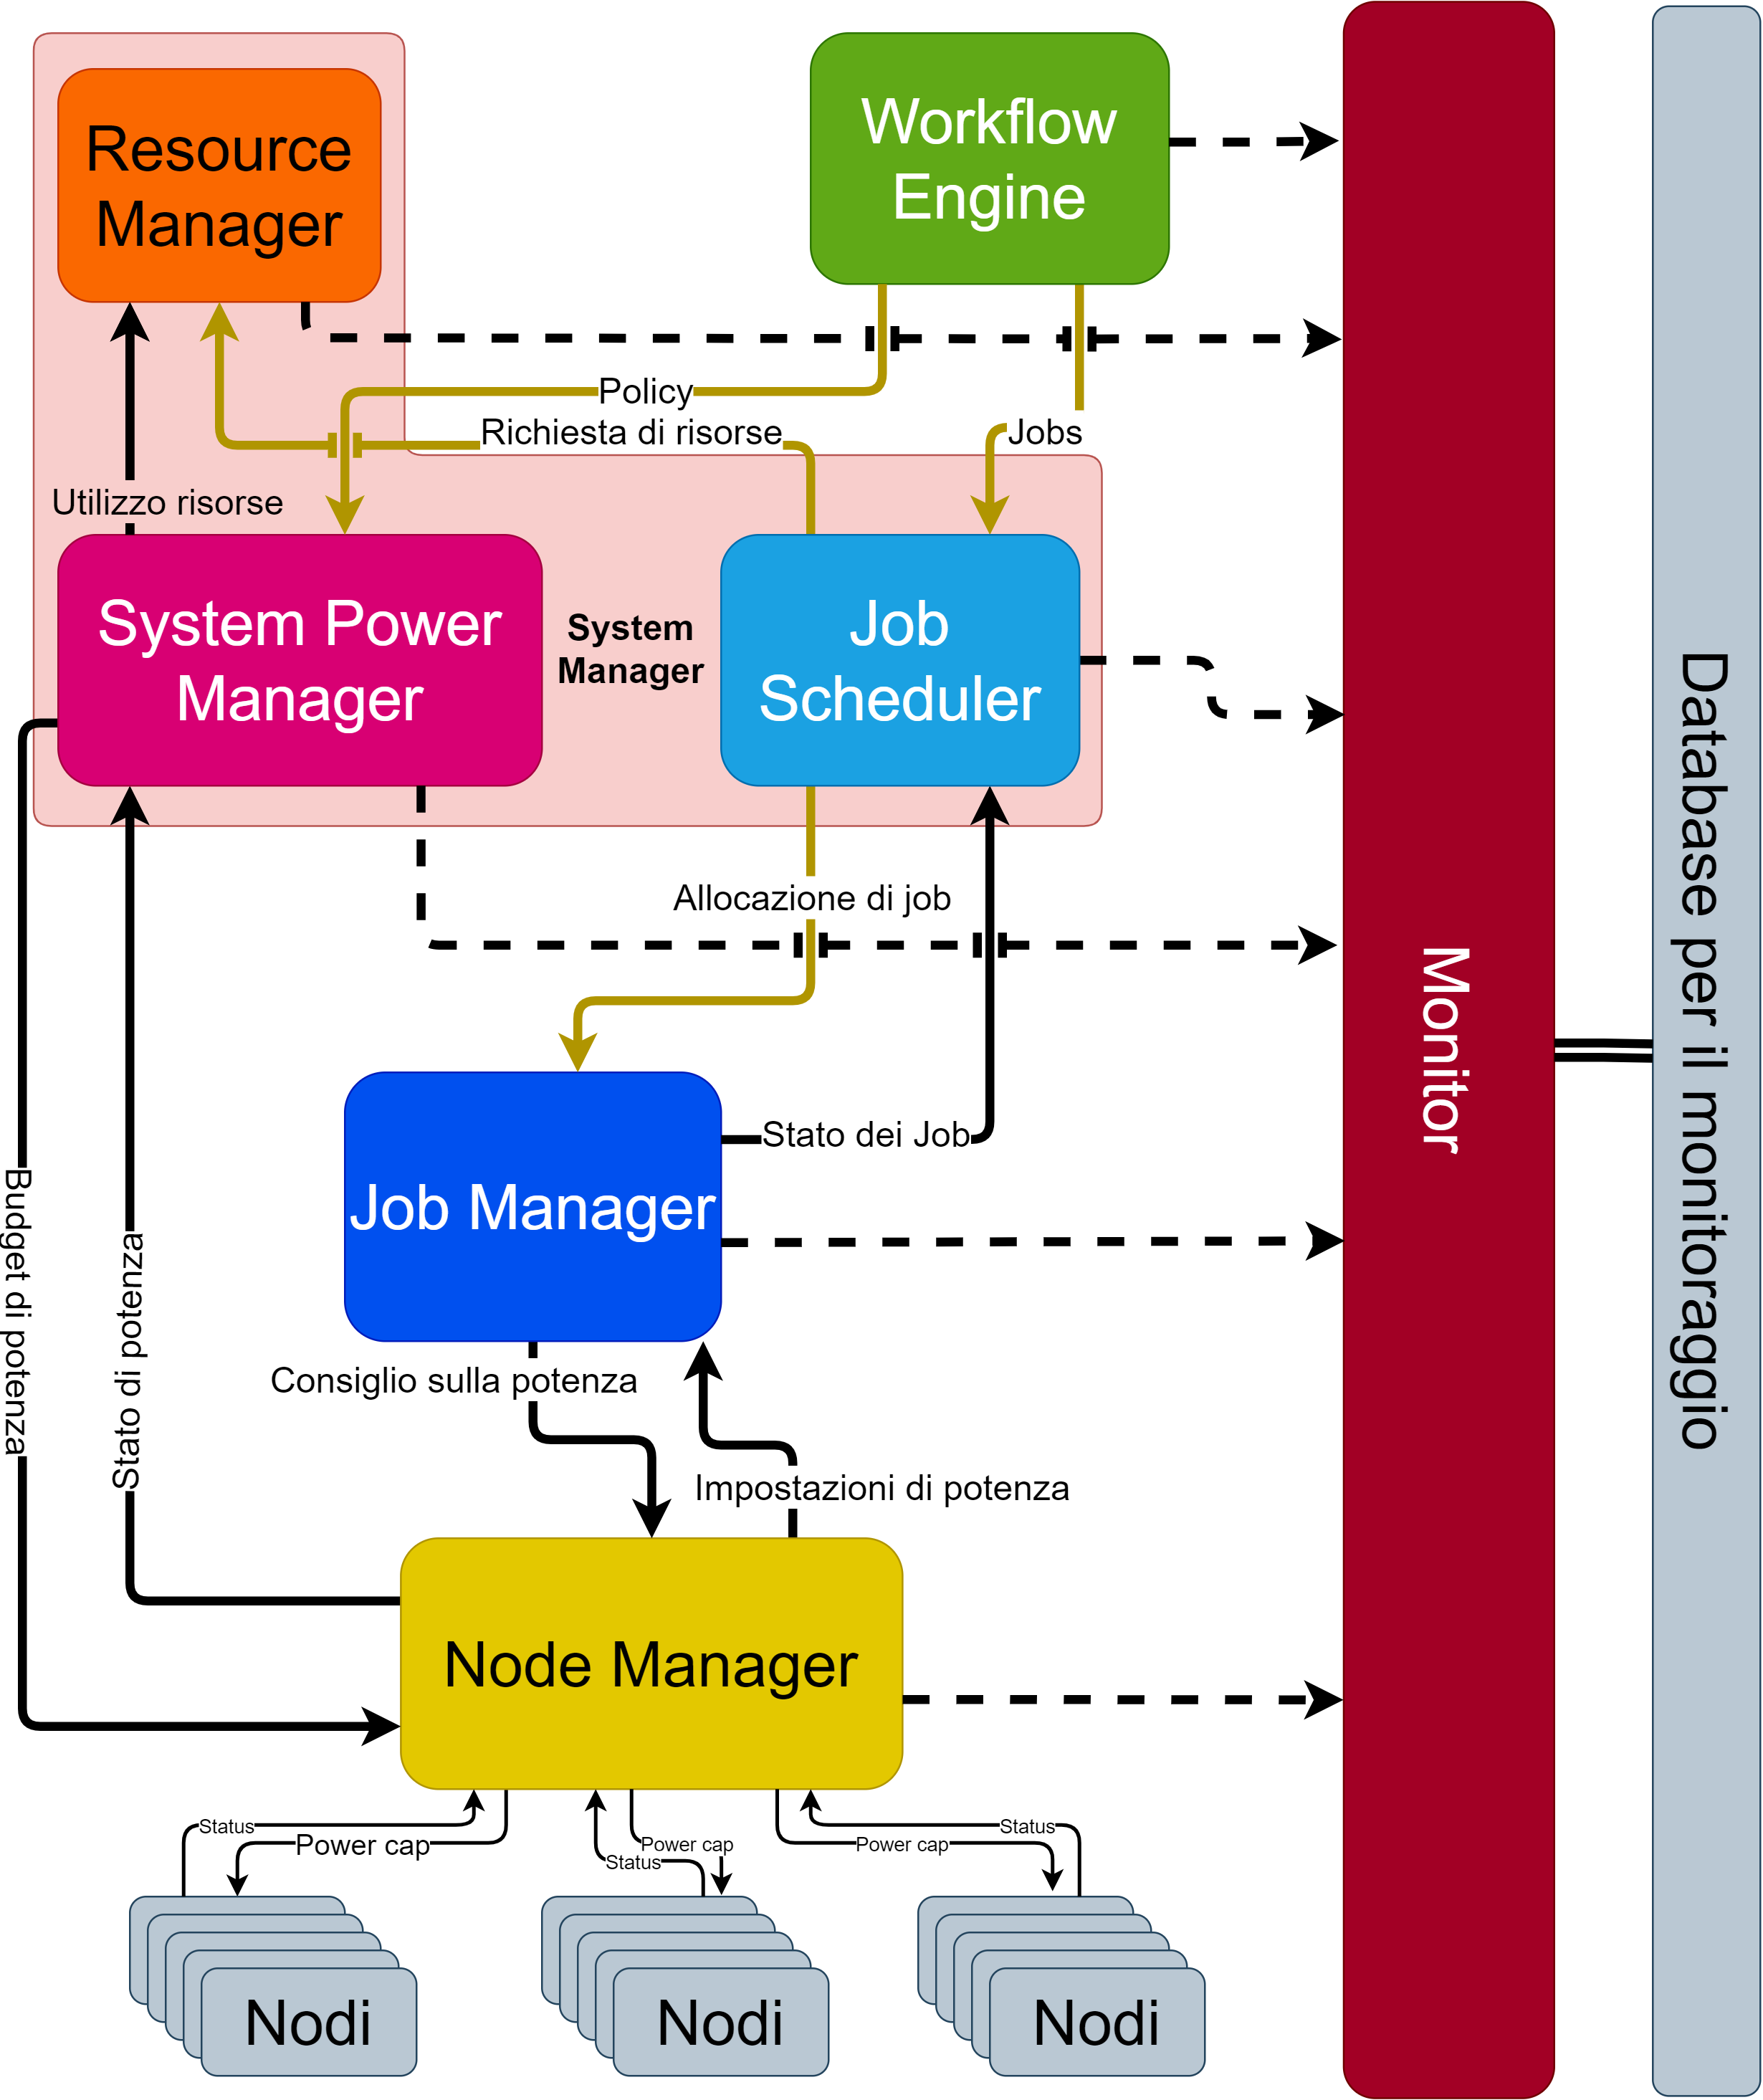
\includegraphics[width=\textwidth]{img/SchemaPowerStack.drawio.png}
    \caption{Modello di power stack}\label{fig:minpowerstackscheme}
\end{figure}


